%!TEX root = ../abgabe.tex

\section{Gestaltungsregeln und Hinweise}

Geschrieben von: Saulius A

In diesen Kapitel werden verschiedene Gestaltungsprinzipien vorgestellt, die bei einer Gestaltung und Entwicklung von Applikationen und Webseiten (später meist nur Applikationen) für einem mobilen Kontext zu beachten sei. Viele der vorgestellten Prinzipien sind nützlich für eine breite Palette von Geräten, die in mobilen Kontext benutzt werden können. Es wird aber vorwiegend auf die auf die Gestaltung von der Applikationen für die Smartphones in Betracht gezogen. Am Ende dieses Kapitels, werden Gestaltungshinweise für die Entwicklung der Applikationen in Wearable Computing Kontext vorgestellt, die auch spezielle Anforderungen erfühlen müssen.

Seit der stetige Verbreitung von Smartphones und mobilen Geräten in alltäglichen Leben, steigt auch die Benutzung von Applikationen in mobilen Kontexten. Dabei stoßen viele der Benutzer, die auf ihren mobilen Gerät auf vorhandene Dienste zugreifen wollen meistens auf viele Usability Probleme. Solche Probleme liegen nicht nur in Inhaltsstruktur oder Visuelle Kommunikation, sondern auch in der Funktionen, die Dienste anbieten. Es liegt meistens daran, dass die vorhandenen Dienste für die Erledigung von Aufgaben auf einem stationären Rechner gestaltet wurden. Dabei beachten die Dienste nicht die Einschränkungen sowie auch Vorteile, die der mobiler Kontext und Geräten für ihn für den Benutzer bedeuten.

Bei schon vorhandenen Applikationen muss meistens nicht nur der Design, sondern auch die Funktionalität der Applikationen sowie die Benutzungsumgebung und Benutzer Intentionen angepasst werden. Jakob Nielsen erwähnt in seinem Artikel \footnote{http://www.nngroup.com/articles/mobile-site-vs-full-site/, es ist ein Ausschnitt aus Bericht "Mobile Website and Application" http://www.nngroup.com/reports/mobile-website-and-application-usability/} die Hauptideen, die für eine Optimierung der Vorhandenen Webseiten für mobile Nutzung helfen sollte:
\begin{itemize}
	\item \textbf{Beschneide Funktionalität}. So sollen nur Funktionen angeboten werden, dessen Anwendungsfall in mobilen Kontext passt
	\item \textbf{Beschneide Inhalt}, um die fülle von Text zu verkleinern und um die sekundäre Informationen in anderen Seiten zu verlagern
	\item \textbf{Vergrößere Elemente der Benutzeroberfläche}
\end{itemize}

Es wird viel darüber gestritten, ob es die Ideen von Jakob Nielsen einen Richtiger Weg für die Entwicklung von Applikationen für mobilen Geräten zeigt\footnote{http://www.netmagazine.com/opinions/nielsen-wrong-mobile}. So wird es vorgeworfen, etwa dass man statt nur Beschneidung der Funktionalität auch auf die Zusatzmöglichkeiten der mobilen Geräten berücksichtigen sollte. In diesen Kapitel wird die Ideen von beiden seiten betrachtet. So werden die Möglichkeiten der Informationsaufbereitung in Kapitel \ref{sec:Informationsaufbereitung} vorgestellt, und sollte bei der Erstellung von Applikationen für mobilen Kontext erwogen werden. Als weiteres werden die Anforderungen an den Bedienelementen sowie die Arten der Interaktion in Kapitel \ref{sub:Benutzerschnittstellen}vorgestellt. Da auch Dienste bestimmte Anforderungen erfühlen sollten, werden diese in Kapitel \ref{sub:gestaltung_von_diensten}vorgestellt. In allen Kapiteln werden keine generelle Gestaltungsprinzipien wie Gesetze der Nähe vorgestellt, sondern nur auf die Konzentriert, die für den mobilen Geräten sowie mobilen Kontext als wichtig erschienen.

\subsection{Bedienelementen und Interaktion}
\label{sub:Benutzerschnittstellen}

Es gibt eine Vielzahl von Smartphones, sowie deren Eingabe- und Ausgabearten. Der Benutzer kann meinstens mit einem Gerät entweder über einem Touchscreen, Tastatur, Ziffernblock, Trackpoint usw. Interagieren. Jeder diese Eingabegarten hat einen anderen Charakter, daher werden die folgende Prinzipien mehr für Eingabe mittels Touchscreen ausgerichtet.

In diesen Kapitel wird über die wichtigen Prinzipien bei der Gestaltung von Benutzeroberfläche, sowie die Interaktion in mobilen Kontext berichtet

\subparagraph{Bedienelementen auf der graphische Oberfläche} 
\label{subp:gro_ere_interface_elementen}

Die Einschränkungen durch einen kleinen Bildschirm auf einen Smartphone müssen bei der Erstellung von Grafischen Benutzeroberflächen besonders beachtet werden. So muss bei der Erstellung von Elementen die physischen Eigenschaften des Fingers beachtet. Laut einer Stunde von MIT Touch Lab, ist der Menschliche Finger im Durchschnitt etwa 10-14mm breit, und die Fingerspitze etwa 8-10 mm\cite{Srinivasan:2003uu}. In der Studie von Pekka Parhi et.al \cite{Parhi:2006gh} wurde erforscht welche optimale Größe von Bedienungselementen für eine Einhändige Daumeninteraktion ist. So wurde erfahren, dass es keine signifikanten Unterschiede in der Bedienung von Elementen bei einer größe ab $>$ 9,5 \textit{mm} bei getrennte, sowie $>$ 7.7 \textit{mm} bei seriellen Erledigungen der Aufgabe existieren. Auch die Hersteller von mobilen Betriebsystemen schlagen ähnliche Maße für Bedienelementen vor. Apple setzt eine Mindestgröße von 44 x 44 Punkten \cite{Apple}, Microsoft 7 \textit{mm} oder 26 \textit{px}\cite{lukeGUI} für Elementen voraus.

Nicht nur die Größe der Elemente, sondern auch der Zwischenabstand zwischen diese ist wichtig für eine benutzerfreundliche Bedienung der Anwendung. Wie man schon in Bild (HIER FOTO mobilefirst 79) zu sehen ist, muss hier der Benutzer sich anstrengen, um den richtigen Element in der Liste auszuwählen. Auch ein mögliches unbeabsichtigtes Anklicken von "Cancel" Bedienelement kann in Beispiel (BILD) verhersehbar sein. So ist es empfohlen einen Zwischenabstand, so genannten Whitespace, zwischen Bedienenlementen zu benutzen. Solche Abstände sollten mindestens von 2\textit{mm} oder 8\textit{px} betragen\cite{lukeGUI} um die unbeabsichtigte Einhaben zu vermeiden.

\subparagraph{Anordnung von Elementen} 
\label{subp:anordnung_von_elementen}

Eine richtige Auslegung von Elementen in der Benutzeroberfläche, kann den Benutzer helfen ohne Kraftaufwand oder Wechsel von der Haltung des Geräts auf die wichtigen Funktionen zuzugreifen. Eine Einhändige Interaktion mit den Smartphones sollte ermöglicht werden, um den Bedienen der Applikation in mobilen Kontext zu erleichtern. So wird empfohlen die wichtigen Elemente so auszulegen, dass sie leicht mit den Daumenfinger erreicht werden \cite[Seite 209]{mobileFrontier}. Da es etwa 70 bis 90 $\%$ der Menschen Rechtshändig sind, ist es laut \cite[Seite 72]{mobileFirst} verbreitet die Elementen  nach der Bequemlichkeit für den Daumenbewegung in 3 Bereichen auszulegen, wie im Bild~\ref{fig:rechtsPositioning} zu sehen sind. Da es aber keine Benutzer benachteiligt werden sollten wurden in diese Arbeit anhand der Ergebnisse aus der Studie \cite{Park:2010tu} die Bereiche verändert und der Resultat im Bild~\ref{fig:forallPositioning}\cite[Seite 72]{mobileFirst} präsentiert.

Die Bedienungselementen, die sehr oft in der Interaktion benutzt werden, sollten in Bereich "Leicht" platziert werden, da sie leicht mit den Daumen erreicht werden können. Die Elemente in "Ok" Bereich, brauchen schon ein wenig mehr Daumenbewegung und bieten weniger Komfort für den Anwender. Der Bereich "Greifen" muss meistens mit eine Greifbewegung erreicht werden, und bietet sich für Navigationselementen, da sie nicht so oft verwendet werden.

\begin{figure}
	\centering
	\begin{subfigure}[b]{0.3\textwidth}
		\centering
			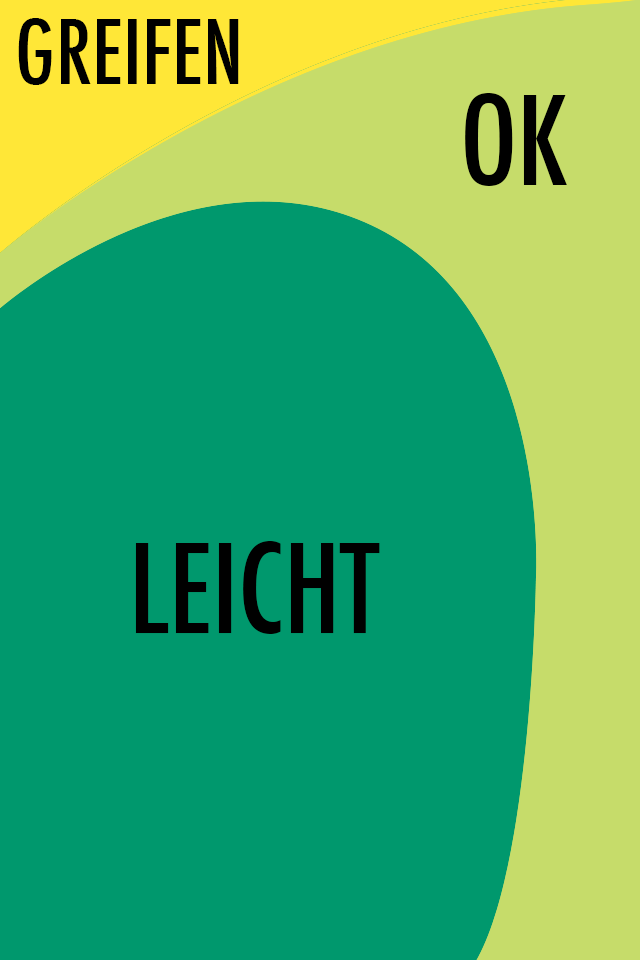
\includegraphics[width=1\textwidth]{img/anordungDerElementeSimple.png}
			\caption{Für Rechtshänder\linebreak}\label{fig:rechtsPositioning}
	\end{subfigure}
	\begin{subfigure}[b]{0.3\textwidth}
		\centering
			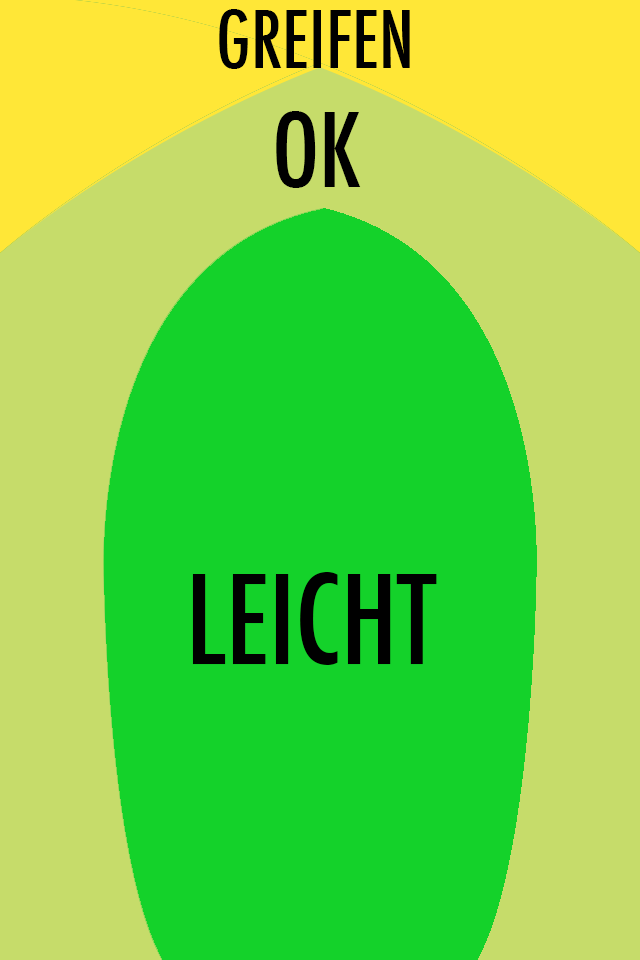
\includegraphics[width=1\textwidth]{img/anordungDerElementeForAll.png}
			\caption{Für Links- und Rechthänder, angepasst anhand Studie \cite{Park:2010tu}}\label{fig:forallPositioning}
			
	\end{subfigure}
	\caption{Positionierung von Elementen}\label{fig:elementPos}
\end{figure}


\subparagraph{Vorsicht bei NUI} 
\label{subp:benutze_nui}

Die meisten Touchgeräten bieten eine direkte Eingabe, mit denen Naturelle Gesten möglich sind. Dabei läuft man in der Gefahr, den Anwender die Bedienbarkeit der Applikation zu erschweren anstatt zu erleichtern. In mobilen Kontexten können viele Situationen auftreten, in den man nur eine Hand bzw. ein Finger für den Bedienung des Smartphones benutzen kann. Dadurch werden Gesten, für deren Ausführung mehr als ein Finger nötig ist, nicht brauchbar. So sollte man über alternative Möglichkeiten zur Ausführung solcher Interaktionen nachdenken. Wie in Beispiel im Bild~\ref{fig:nuibsp} bietet die vorgeschlagene Benutzeroberfläche\footnote{Ausschnitt aus OpenSteetMap.com} als Alternative für die Pinch oder Spread Gesten einen Schaltknopf. Beim Drücken dieses Schaltknopfes, kann die Karte verkleinert oder vergrößert. 

\begin{wrapfigure}{r}{0.5\textwidth}
	\begin{center}
	
	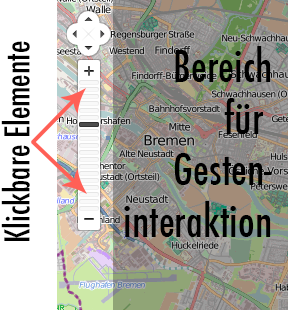
\includegraphics[width=0.3\textwidth]{img/NUIbsp.png}
	\caption{Alternative Interaktionsmöglichkeiten}\label{fig:nuibsp}
\end{center}
\end{wrapfigure}

\subparagraph{Designe für wechselde Umgebungen} % (fold)
\label{subp:designe_f_r_au_eneinsatz}

Bei Bewegungen, ändert sich die Umgebungen. Und die Umgebungen haben verscheide Eigenschaften. So wird zum Beispiel ein Benutzer der aus ein helligen Tag ins dunklen Kinosaal geht und dabei versucht weiter sein Smartphone zu benutzen,  von der starke Leuchtkraft des Bildschirms überblendet. Daher ist es zu Empfehlen, Bedienelemente leicht erreichbar zu platzieren, um die Helligkeit ( vgl. \cite[ff Seite 418]{mobileInteraces}) zu regulieren oder die Farben der Benutzeroberflächen zu invertieren. Auch an andere Auswirkung der wechsel der Umgebungen sollte berücksicht werden.
\newline

In diesen Kapitel, wurden die paar der wichtigen Prinzipien von Gestaltung der Benutzeroberfläche für mobilen Kontext erwähnt. So sollte der Gestallter solcher Oberflächen wissen über die Grenzen des Fingers, sowie wie man Elemente auf der Oberfläche belegen muss, um eine bequeme bedienung zu ermöglichen. Als weiteres wurde auf die Gefahren bei wechselnde Umgebungen informiert sowie möglichen Eingrenzungen bei NUI. In nächsten Kapitel wird die Prinzipien für die Informationsarchitektur präsentiert.

\subsection{Informationsarchitektur}
\label{sec:Informationsaufbereitung}


Menschen in mobilen Kontexten haben viele Anforderungen an der Applikationen die anders sind als für stationären Arbeitsplätzen. Um gut benutzbare Software für solchen Szenerien zu entwickeln, ist daher wichtig die Aktionen sowie Verlangen von Benutzer zu wissen und zu berücksichtigen. Man sollte wissen, wieso und wann benutzen die Anwender den Smartphone in mobilen Kontext. Eine Einteilung von Benutzer kann dabei helfen, spezielle wünsche, sowie Erwartungen an der Applikationen herauszufinden.

Die Einteilung, kann laut Google anhand Anwenderverhaltens eingeteilt werden. So wurden drei Gruppen identifiziert: "urgent now", "repetitive now", "bored now"\cite{googleUsers}. Benutzer der Gruppe "Urgent now" wollen ein wenig Informationen schnell bekommen, wie etwa die Adresse des Arztes oder Buchladens. Anwendungen, die diesen Verlangen erfühlen sollten, sollten etwa mit der Hilfe von Ortsdaten, wo sich der Benutzer befindet die suche initiierten. So sollen die Ergebnissen schnell und ohne bewusste Benutzereingabe geliefert werten. Benutzer der Gruppe "Repretitve now" wollen gleiche Art der Informationen immer wieder aufrufen, wie etwa Wettervorhersage oder Aktienkursen. Solche Informationen sollten schnell sichtbar oder aufrufbar sein. Benutzer die der Gruppe "bored now" gehören, sind im Zustand, wo sie viel Zeit für Interaktion mit den Gerät haben, etwa in Empfangshalle von Flughafen oder im Öffentlichen Verkehrsmittel. Die Erwartungen der Benutzer in diesen Situationen ähnelt den Benutzer, die mit einem stationären Rechner ihre Aufgabe erledigen, aber sie verfügen anderen Ausgabe- sowie Eingabegeräten und können jederzeit für unbestimmte Zeit von der Bedienung des Gerätes unterbrochen werden. So kann in "bored now" Szenario Aufgaben erledigt werden, die mehr Zeit und kognitiven Auslastung voraussetzen, als bei "urgent now" oder "repetitive now".

Die Vorgestellte Einteilung ist zwar nützlich, aber nicht gründlich genug. Daher kann man eine Einteilung anhand Arten der Interaktion statt den Benutzerverhalten benutzen. Sie ist mehr hilfreich, um einem Fokus auf die Gestaltung von den Informationsarchitektur zu haben. So können die mobile Arten der Interaktionen im mobilen Kontext in vier Kategorien eingeteilt werden( anhand \cite[Seite 50]{mobileFirst}):

\begin{itemize}
 	\item[Suche (wichtige Information, lokal)] Ich brauche schnell eine Antwort zu meine Frage. Sie kann die auch oft wiederholt vorkommen, und ist bezogen auf meine Position in der Welt
 	\item[Erforschen/Spielen (gelangweilt, lokal)] Ich habe Zeit, und will eine kurze Ablenkung
 	\item[Einchecken/Status (Wiederholung/kleine Aufgaben)] Irgendwas ändert sich, und will ich das Neuste wissen oder teilen
 	\item[Editieren/Kreieren (plötzliche Veränderungen/ kleine Aufgaben)] Ich muss was schnell erledigen
 \end{itemize} 

Diese Kategorisierung anhand Arten Der Interaktion von Benutzer, hillft dessen Bedürfnissen zu spühren und somit eine geeignete Applikation zu gestalten. Wenn man etwa eine Applikation für Wetter gestalten, so kann man die Benutzer mit Intentionen der Kategorie \textbf{Suche} bedienen, in den man auf den ersten Bildschirm den Wetter anhand der Position von Benutzer anzeigt. Um die Gruppe "Einchecken/Status" zu bedienen, sollte man etwa die Möglichkeit bieten den Benutzer Wetter für von ihn gespeicherten Städten anzuzeigen. Die Gruppe "Erforschen/Spielen" zu bedienen, sollte man Zusatzfunktionen wie 14 Tage Wetterbericht, Regenkarte und andere Funktionalität anbieten, die mit Hilfe von Navigation von Anfangsbildschirm erreicht werden können.

Es gibt auch generelle Ideen, die eine vorhandene Applikation für den mobilen Kontext optimieren oder neue Applikation gestallten oder umorganisieren kann. In folgenden Unterkapiteln wird die wichtigsten Hinweise präsentiert. 

\subparagraph{Mach es schlank} 
\label{subp:entferne_das_fett}

Wie schon in der Einleitung von diesen Kapitel erwähnt wurde, empfehlt Jakob Nielsen die Informationsangebote auf mobilen Webseiten zu reduzieren. So soll unnötiges Text entweder auf anderen Seiten verlagern, oder am besten wegstreichen. Mann soll es so machen, da es auf einen kleinen Gerät ist schwieriger zu lesen\cite[Seite 102]{Nielsen:2012wj}. Es liegt an den Zwang zu blättern wegen kleine Anzeige größe. So braucht der Benutzer mehr Zeit für Lesen , sowie ist es ihm schwieriger auf anderen Textpassagen zurückzugehen.

Auch die Funktionsangebot soll für den mobilen Kontext angepasst werden. Als Beispiel kann hier die Amazon Webseite dienen (siehe Bild~\ref{fig:amazon}. So wird bei der Auswahl von einen Produkt auf der mobile Webseite von Amazon, ein Bild, ein Preis und Funktionalität für sofortigen Kaufen oder Merken angeboten. In vergleich zu eine Desktop Webseite ist der Funktionsangebot reduziert (siehe Bild~\ref{fig:amazonFull}). Um mehr Informationen über Produkt zu bekommen, was für die Gruppe "Erforschen/Spielen" wichtig wäre, kann mit Hilfe sekundäre Seiten gelöst werden.

\begin{figure}
	\centering
	\begin{subfigure}[b]{0.3\textwidth}
		\centering
		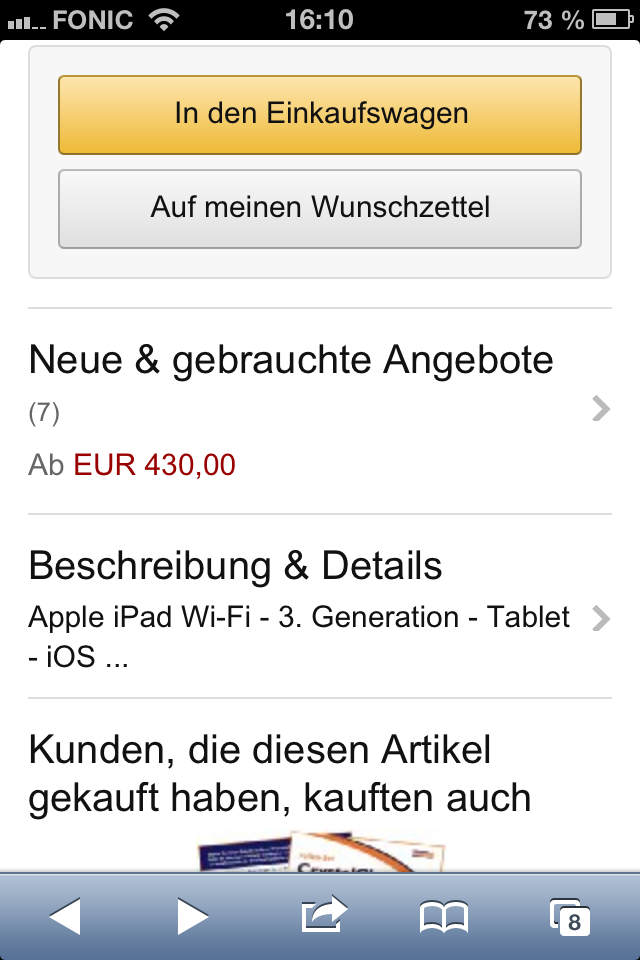
\includegraphics[width=1\textwidth]{img/amazon.png}
		\caption{Mobile Webseite}\label{fig:amazon}
	\end{subfigure}
	\begin{subfigure}[b]{0.6\textwidth}
		\centering
		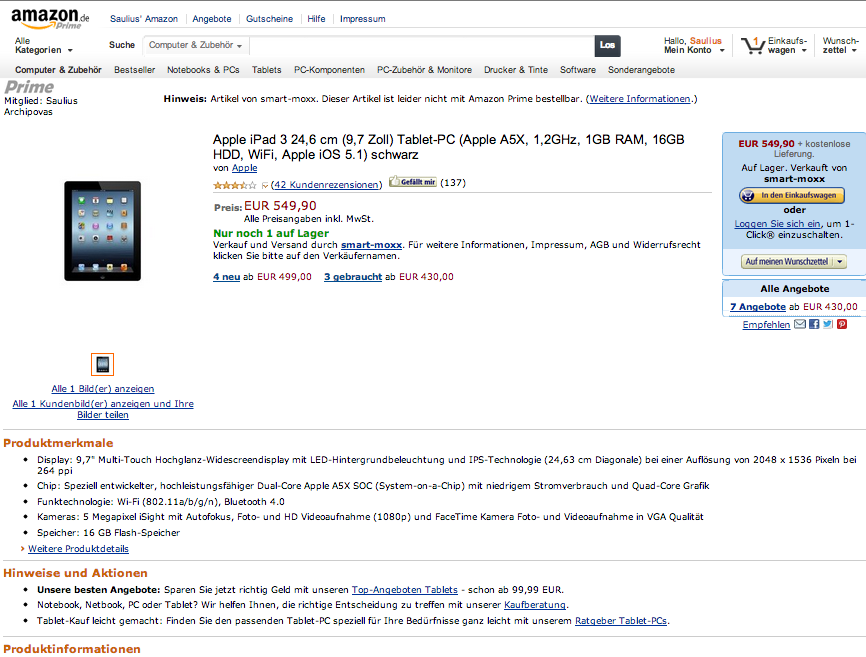
\includegraphics[width=1\textwidth]{img/amazonFull.png}
		\caption{Normale Webseite}\label{fig:amazonFull}
	\end{subfigure}
	\caption{Webseiten von Amazon}\label{fig:amazonSites}
\end{figure}

\subparagraph{Mehr Inhalt, weniger Navigation} 
\label{subp:entferne_das_fett} 

Auch die Konzentration auf den Inhalt und nicht die Navigation sollte in mobilen Kontext bevorzugt werden\cite[Seite 52]{mobileFirst}. So hat der Besucher der Kategorie "Suche" oder "Erforschen/Spielen"  wenig Zeit um Inhalt zu konsumieren, daher sollte er nicht mit eine Sitemap überfordert werden um zu überlegen wo er jetzt hin soll. Als gutes Beispiel dient hier Youtube App, die einen bequemen direkten Einstieg für Konsum ausgelegt ist. Es werden Videos für den Benutzer vorschlägt (siehe Bild~\ref{fig:youtube}), was einen schnellen Inhaltskonsum verbessert. Die Seitennavigation ist unter nur einen Bedienknopf unterlegt, und somit spart auch Platz auf den Benutzeroberfläche.

\begin{wrapfigure}{r}{0.5\textwidth}
	\begin{center}
	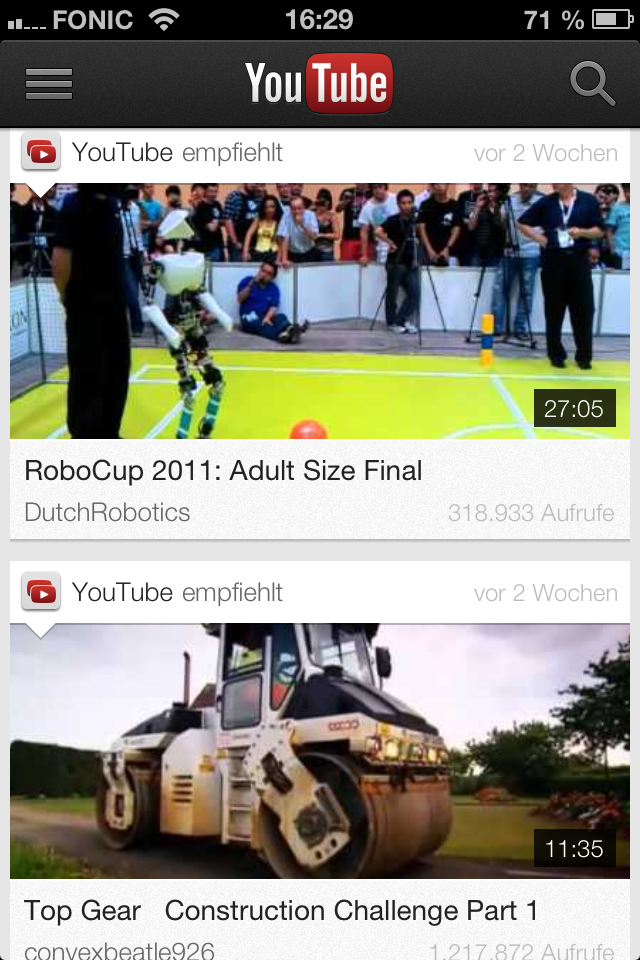
\includegraphics[width=0.3\textwidth]{img/youtube.png}
	\caption{Youtube}\label{fig:youtube}
\end{center}
\end{wrapfigure}

\subparagraph{Schneller Zugriff auf wichtige Informationen} 
\label{subp:subparagraph_name}

Wie im Szenario "Suche", will der Benutzer nicht immer in das Innenleben von Programmen eintauchen, nur um kleinen wichtigen Bruchteil der Information zu gewinnen. Deshalb sollte man wesentliche Informationen schon beim einem Überblick erkennbar sein(vgl. \cite[Seite 54]{mobileFrontier} und \cite{Neil:2012uf}). Als Beispiel dient hier iPhone Startansicht. Hier wurden die Piktogramme so gestaltet, dass sie wichtige Information selbst beinhalten. So beinhaltet etwa die Piktogramm von iOS Kalender den heutigen Tag(siehe Beispiel in Bild~\ref{fig:iconIos}), oder Errinerungs App Hinweiß auf Anzahl der Errinerungen.

\begin{wrapfigure}{r}{0.5\textwidth}
	\begin{center}
	
	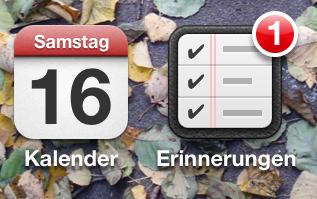
\includegraphics[width=0.3\textwidth]{img/iconIos.png}
	\caption{Schneller Zugriff auf Informationen}\label{fig:iconIos}
\end{center}
\end{wrapfigure}

\subparagraph{Reduziere Kognitive Aufgaben} 
\label{subp:reduziere_kognitive_aufgaben_}

In den mobilen Kontext ist der Benutzer meistens mit verschiedene Aufgaben beschäftigt, so ist auch die Verfügbarkeit der Aufmerksamkeit viel weniger, als etwa in Büro. Bei Gestaltung von Applikationen, mit denen in mobilen Kontexten gearbeitet werden soll, sollte es immer berücksichtigt werden. So soll Anwendungen entstehen, die das unnötige Denken abnimmt. So können die typischen "Wo bin ich" Hinweisen angezeigt werden, oder eine klare Strukturierung der Navigation sowie des Layouts viel helfen. 

Auch die Elementen der Benutzeroberfläche muss den Benutzer nicht überfordern. So sollten unnötige Animationen in eine Anwendung vermieden werden, da sie den Anwender unnötig ablenken oder für längere Zeit unnötig seine Aufmerksamkeit lenken können. Solche Ablenkungen können sogar auch den Benutzer gefährden, da er von seine Tätigkeiten in Realen Welt abbringen und somit sogar zu Unfällen führen können (vgl. \cite{Nasar:2008cc})

\subparagraph{Reduziere Navigationstiefe} 
\label{subp:reduziere_das_w_hlen}

Eine Hierarchisch aufgebaute Navigation ist ein viel benutztes Navigationsmuster in Webseiten sowie Desktop Applikationen. Dieses Muster sollte auch für Applikationen für mobilen Kontexten benutzt werden. Dabei muss beachtet werden dass die Tiefe der Navigation nichts zu groß halten wird. Mit jede weitere Tiefe muss der Benutzer sich mehr Erinnern und Abrufen, was in mobilen Kontext schwierig wird, weil er oft abgelegt word und meistens nur 4 Sekunden Aufmerksamkeitsspanne auf die Applikation hat\cite{Oulasvirta:2005vn}. Bei nicht mobilen Kontexten wurde beobachtet, dass solche Navigationen eine Fehleranfälligkeit von 4\% auf 34.0\% bekommt, wenn die Navigationsstruktur von 1 bis 6 erhöht wird (Snowberry at al. Zitiert von \cite{Chae:2004gp}). Diese Beobachtung sollte in Betracht gezogen werden, so oft angewendete Tiefe der Hierarchie von drei Stufen benutzt werden.


\subparagraph{Nutze alternative Ein- und Ausgabequellen}
\label{subp:nutze_alternative_eingabenger_ten}

Die Interaktion mit den mobilen Gerät kann in einem mobilen Kontext durch vieles beeinflusst werden. So kann der Benutzer etwa beim Fahren einen Autos nicht mit der Hand bedient werden, oder der Blick kann nicht immer auf den Bildschirm ausgerichtet werden. So sollen auch andere Ein- oder Ausgabequellen benutzt werden. Es kann bei genannten Beispiel etwa auf die Sprache als Eingabe, sowie Ausgabe dienen. 

Auch die Geolokalisierung kann sehr behilflich sein, um etwa Benutzer Informationen anzubieten bei erreichen eines Bestimmten Ortes, ohne Bewusste Eingabe des Ortes durch den Benutzer . Geolokalisierung kann auch Benutzer helfen, weniger Informationen für eine Suche anzugeben, wenn etwa er nach eine Kaffe sucht. So können schon in voraus Kaffes in Unmittelbare nähe gesucht werden, anstatt den Benutzer explizit nach seinem Ort zu befragen.

Die Benutzung von Status-Led oder Vibration kann Benutzer auf Ereignisse Hinweisen, ohne dass er immer auf den Bildschirm es sehen muss. So kann man in Android Notifications benutzen, um etwa die Status-LED mit bestimmte Farbe und Intervallen blinken zu lassen (vgl. \cite{androidNotApi}). Benachrichtigungen bergen auch viele Gefahren, wenn sie nicht durchdacht benutzt werden. So kann es leicht passieren, dass der Benutzer mit Benachrichtigungen regelrecht überflutet wird und nicht mehr auf Erfüllung seine gewünschten Aufgaben Konzentrieren kann, da er permanent von Benachrichtigungen abgelenkt werden kann.

\subparagraph{Designe für Unterbrechungen und ermögliche eine Fortsetzung}
\label{subp:erm_gliche_eine_fortsetzung}

Im mobilen Kontexten wird der Benutzer oft Unterbrochen in Interaktion mit einem mobilen Gerät oder er hat nicht genügend Zeit seine Aufgaben zu beenden. Es sollten Möglichkeiten angeboten werden die Aufgaben später zu Erledigen. So sollten Benutzereingaben oder der Anwendungszustand nicht zurückgesetzt werden nach bestimmten Zeit, um den Benutzer eine Fortsetzung seiner Aufgabe zu ermöglichen.

Die Hersteller von mobilen Betriebsystemen bieten dafür spezielle APIs, um dies zu ermöglichen. So können Daten beim schließen der Applikation zwischengespeichert werden, um sie nach nächsten Aufruf der Applikation den Benutzer zu ermöglichen seine Arbeit weiterzuführen. Wenn der Benutzer dies nicht wünscht, sollte eine Möglichkeit geben, die Applikation in einen Startzustand mit wenig Interaktion zu setzen.

Außerdem solle man den Benutzer die Möglichkeit geben bei Bestimmten Kontexten Teilaufgaben zu markieren, die dann in "Erforschen/Spielen" Art der Interaktion einteilen kann, erledigt werden können. Als gutes Beispiel dient hier der Dienst "Pocket" \footnote{Vorher als "Read it later" bekannt, http://getpocket.com } Funktionalität. So kann der Benutzer interessante Artikeln, oder Webseiten markieren, uns sie später in alle ruhe durchlesen zu können. Auch als Beispiel konnte ein dienst Dienen, in den man Gerade besuchten Ort markieren, um danach mehr Information über den Ort zu erfahren.

\subparagraph{Fokussiere auf Erfahrungen, die nur mobil auftreten können} % (fold)
\label{subp:fokussiere_auf_erfahrungen_die_nur_mobil_auftreten_k_nnen}

Es wurde vier Kategorien in diesen Kapitel eingeführt, die den Art der Interaktion beschreiben. Die Anwendungen für mobilen Kontext sollten auch diese bedienen, und nicht versuchen einen Stationären Arbeitsplatz zu imitieren. Auch die Erfahrungen, die nur mobil auftreten können, sollten berücksichtigt werden.

Zum Beispiel bei Eine Notiz Applikationen, man würde den Benutzer ermöglichen Lokalisierungsinformationen oder Schnelle Schnappschüsse zu speichern. Oder eine Applikation, die Preisvergleiche macht, sollte eine Barcode-Lesefunktion haben, um den Benutzer bei besuch eines Ladens die Preise zu scannen zu ermöglichen. Auch eine Rabatcoupon Erinnerung bei besuchen eines bestimmten Laden könnte den Benutzer Freude an der Applikation bereiten (vgl. \cite{smartOnline})
\newline

In diesen Teilkapitel wurden die vier Arten der Interaktion, sowie wichtigen Hinweise für Erstellung von Applikationen hinsichtlich ihre Informationsarchitektur. So wurde empfohlen die Applikationen nicht mit Text, Funktionalität und Navigation den Benutzer zu überfordern, sondern mehr auf den knappen und schnell für den Benutzer wichtigen Inhalt zu konzentrieren. In nächsten Kapitel werden die Hinweise über die Gestaltung von Diensten gegeben.

\subsection{Gestaltung von Diensten}
\label{sub:gestaltung_von_diensten}

Nicht nur der Visuelle Design von der Applikation muss für mobilen Einsatz angepasst werden, sondern auch die Dienste, die der Applikation anbietet, den mobilen Einsatz unterstützen. 

Bis jetzt wurden die Kernaufgaben, die mit einem Rechner erledigt werden konnten, mit den Stationären Rechner erledigt. Mit immer mehr verbreitende Benutzung von mobilen Geräten, sollten die Barrieren von Informationsaustausch zwischen den beiden Gerätearten den Benutzer erleichtert werden. Als Benutzer will man eine Möglichkeit Arbeiten die am einen Gerät angefangen wurden, auf anderen Gerät weiterzuführen. Diese Bedürfnisse wurden teils von Mitarbeiter aus der precious design studio analysiert und es wurden sechs Beziehungsmuster von Anzeigen identifiziert, die auch für Gestaltung von Diensten benutzt werden könnten\cite{slideEcosystems}. Es werden Beziehungsmuster Kohärenz, Synchronisation und Gerätemobilität näher betrachtet.

\subparagraph{Kohärenz}

Dienste, die auf einem stationären Rechner laufen, sollten auch die Möglichkeit bieten die Hauptfunktionalität des Dienstes auch auf einen mobilen Gerät zu benutzen. So soll auch eine sofortige Synchronisation zwischen Geräten existieren, um Möglichkeit von Bearbeitung von der Aufgaben des Benutzer auf beliebigen Gerät zu ermöglichen. Dabei sollen die Applikationen an den Eingeschalten des benutzen Gerät optimiert oder erweitert werden.

Als gutes Beispiel dient hier eine Anwendung Evernote, die für Notizen benutzt werden kann. So kann man mit den mobilen Gerät Notizen oder Photos hochhalten, und sie weiter am beliebigen Rechner zu bearbeiten oder umgekehrt. Um die Vorteile von mobilen Gerät auszunutzen, werden etwa Daten von Aufnahmeort zu jede Notiz abgespeichert. Außerdem ist die mobile Applikation für Foto-, Audio- und Videonotizen optimiert. So werden durch abfotografieren von Textpassagen der Text erkannt und ins maschinelles übersetzt. So wird die unproduktive Eingabe eines Textes auf einen mobilen Gerät umgegangen.

\subparagraph{Synchronisation}

Benutzer erwarten zunehmend, dass die digitale Informationen und Daten von überall aufrufbar sein sollten. Dies kann gelöst werden, wenn man die Daten zwischen den Geräten ohne expliziten initiieren durch Anwender synchronisiert. So kann bei Wechsel des Gerätes der Benutzer auf identische Daten zugreifen. 

Als Beispiel dient hier der iCloud von Apple. So kann Termine, Musik, Fotos oder Bücher zwischen den Geräten von den Benutzer synchronisiert und im neusten Stand gehalten werden. Bei den Amazon Kindle Dienst ist es möglich nicht nur gleiche Bücher auf verschiede Geräten zu haben, sondern auch an der gleiche Seite von den Buch das Lesen vorzuführen, die auf anderen Gerät aufgehört wurde.

\subparagraph{Gerätemobilität}

Bei der Interaktion mit den Gerät kann es passieren, dass die Intention des Anwenders, oder etwa die Umgebung so ändert, dass der gerade benutzbare Gerät nicht mehr die Bedürfnisse erfühlen kann, und der Benutzer will die Benutzung von den Medium auf einen anderen gerät auszulagern. Dabei soll den Benutzer geholfen werden, Informationen auf einem Gerät übertragen, verschieben, umschalten, verlagern oder hinterlegen ohne großen aufwand.

Als gutes Beispiel dient hier Apple AirPlay. So kann der Benutzer auf den iPhone oder iPad angefangenen Film oder Musik, auf einem anderen Gerät der AirPlay unterstützt verlagern. So kann sofort der Film auf der Verlagerten Gerät weitergespielt werden, siehe Bild (FOTO)
\newline

In diesen Kapitel wurden drei Muster für die Gestaltung von Diensten für einen mobilen Kontext vorgestellt, die den Benutzer den Wechsel der Geräte erleichtern sollten. In nächsten Kapitel wird über spezielle Anforderung bei Wearable Computing vorgestellt, um einen breiteren überblick über Design in mobilen Kontext zu schaffen.

\subsection{Spezielle Anforderungen bei Wearable Computing} 
\label{sub:wearable_computers}

In forherigen Kapiteln wurden viele 

Wearable Computing, oder Tragbare Datenverarbeitung, ist das Forschungsgebiet, das sich mit den der Entwicklung von tragbaren Computersystemen (Wearable Computers) beschäftigt \footnote{citate aus wikipedia }. So wird versucht alltägliche Aktivitäten oder Bedürfnisse des Benutzers  von der Computersysteme zu erleichtern oder sogar ermöglichen, dabei aber tritt der Computersystem im Hintergrund. Die Geräte können beliebige Form sein und Funktion erfühlen: von eine Armbanduhr, die ähnlich den Smartphone funktioniert \footnote{http://www.zeit.de/digital/mobil/2013-01/smartwatch-wearable-computer} bis einem  Ring, der die Pulsrate sowie Sauerstoffgehalt in Blut misst \footnote{http://www.sciencephoto.com/media/349431/view}.  Um eine kurze Einführung in Gestaltungsprinzipien im Wearable Computing zu ermöglichen, wird auf die Benutzung von Wearable Computing in Arbeitsumfeld und die Forschung die im TZI Wearable Labs begrenzen und auf die Head-Up-Display (HUD) Ausgabegeräten beschränkt.

Wearable Computing kann unter auch arbeiten in Industrie (Wartungs-, Lagerarbeit), Gesundheitspflege und anderen Bereichen erleichtern \cite{Witt:2006hi},\cite{Lawo:2008gg}). So besteht eine typische Arbeitskleidung aus einen HUD, eine Tragbare Tastatur sowie eine Handschuh mit Steuerungskomponenten. Die Ausgabe von den Computern kann mittels eines Displays in einem HUD benutzt werden, und die Eingabe mittels eine Tastatur sowie eine Steureungshandschuh erfühlt werden. Die physikalischen grenzen der Auge, also die Möglichkeit von eine Fokussierung auf Objekten ab der Entfernung von etwa 20 cm, also ihre Auflösung sowie die Mögliche Entfernung von HUD Displays, ergeben eine Einschränkung der möglichen visuellen Darstellung von GUI Komponenten. 

Anders als in stationären Arbeitsumfelder, wo meistens nur eine Hauptaufgabe am einem Rechner bearbeitet wird, werden in Wearable Computing erwartet, dass der Benutzer zwei Aufgaben erfühlt \cite{Witt:2006hi}. Diese Aufgaben können ins Primäre und Sekundäre Aufgaben eingeteilt werden. Die Primäre Aufgabe besteht meistens aus einer Interaktion mit dem Umwelt, etwa drehen einer Schraube oder Scannen eines Paketes. Primäre Aufgaben können durch Benutzung des tragbaren Computersystemen erleichtert werden, die als sekundären Aufgaben unterteilt werden können. Sekundären Aufgaben wären etwa Bestätigung von Einschrauben einer Schraube oder zeigen einer visuelle Information über gerade eingescannten Paket. Falls eine sekundäre Aufgaben existiert und erledigt werden muss, sollen dabei der Benutzer nicht zu sehr von der Primären aufgaben ablenkt werden. Erstens man muss nachdenken wie er auf der sekundäre Aufgabe aufmerksam gemacht werden muss, zweitens wie soll die Interaktion mit den Computer erfolgen. Um die Aufmerksamkeit des Benutzers auf die Sekundäre Aufgabe zu bekommen, können 4 Benachrichtigungssysteme benutzt werden: "sofortige", "verhandelbare", "vermittelte" und "geplante" \cite{McFarlane:1999um}\cite{Nilsson:cq}. Bei der sofortige Benachrichtigung, wird der Benutzer sofort informiert über neu Information. Solche Benachrichtigungen sind etwa nützlich bei der Betreuung von Auszubildenden in Autowerkstätten durch den Computer eingesetzt werden. So kann anhand eines Arbeitsschritts, die benötigte Werkzeuge auf den HUD angezeigt werden. Oder wenn eine Schraube am Falschen Ort befestigt wurde, den Benutzer sofort zu informieren. Bei der verhandelbare Benachrichtigungssysteme wird der Benutzer informiert auf seinem HUD über einen Ereignis, und der Benutzer darf entscheiden ob er auf dieses regieren will. So kann etwa beim eintreffen neue Pakete im Lager der Lagerarbeiter informiert werden, und somit entscheiden ob er diese Tätigkeit sofort erledigen will. Bei vermittelte Benachrichtigungen, können andere Arten der Ausgabe für Benachrichtigungen verwendet werden, die nicht so aufdringlich sind wie anzeige auf einem HUD. So kann etwa ein Audiodatei abgespielt werden, die den Benutzer informiert über einen Ereignis. Falls der Benutzer auf ihn Reagieren will, kann es mittels einen Eingabegerätes es starten. Bei der "geplante" Benachrichtigungen werden die Aufgaben  akkumuliert und in festgelegten Intervallen Aufgaben angezeigt werden. In der Studie \cite{Nilsson:cq} wurde der "geplante" Benachrichtigungssysteme besser abgeschnitten bei der Effizienz sowie auch der subjektiver Meinung der Probanden.


In diesen Kapitel wurde mehrere Hinweise, die für Gestaltung von Diensten, Benutzeroberflächen sowie Funktionalitäten für Anwendungen, die in mobilen Kontext benutzt sollten erläutert. In nächsten Kapitel wird eine Beispielanwendung vorgestellt und analysiert.

